\documentclass[10.5pt,notitlepage]{article}
\usepackage[utf8]{inputenc}
\usepackage{amsthm}
\usepackage{amsmath}
\usepackage{amsfonts}
\usepackage{mathtools}
\usepackage{amsmath,amssymb}       
\usepackage{enumitem}   
\usepackage{enumerate}
\usepackage{verbatim} 
\usepackage{bbm}
\usepackage[backend=biber,style=apa]{biblatex}
\usepackage{csquotes}
\DeclareLanguageMapping{spanish}{spanish-apa}
\urlstyle{same}
\addbibresource{refer.bib}
\usepackage{etoolbox}
\patchcmd{\thebibliography}{\section*{\refname}}{}{}{}
\usepackage{hyperref}
\usepackage{booktabs}
\renewcommand{\qedsymbol}{$\blacksquare$}
\usepackage{makecell}
\usepackage[spanish]{babel}
\decimalpoint
\usepackage[letterpaper]{geometry}
\usepackage{mathrsfs}
\newenvironment{solucion}
  {\begin{proof}[Solución]}
  {\end{proof}}
\pagestyle{plain}
\usepackage{pdflscape}
\usepackage[table, dvipsnames]{xcolor}
\usepackage{longtable}
\usepackage{tikz}
\def\checkmark{\tikz\fill[scale=0.4](0,.35) -- (.25,0) -- (1,.7) -- (.25,.15) -- cycle;} 
\usepackage[bottom]{footmisc}
\usepackage{hyperref}
\usepackage{float}
\usepackage[utf8]{inputenc}
\usepackage{placeins}
\DeclareMathOperator{\Tr}{Tr}
\DeclareMathOperator{\diag}{diag}
\DeclareMathOperator{\argmax}{argmax}
\DeclareMathOperator{\argmin}{argmin}
\newcommand{\PP}{\mathbb{P}}
\newcommand{\Bb}{\mathcal{B}}
\newcommand{\RR}{\mathbb{R}}
\newcommand{\Ff}{\mathcal{F}}
\newcommand{\Ss}{\mathcal{S}}
\newcommand{\Aa}{\mathcal{A}}
\newcommand{\Jj}{\mathcal{J}}
\newcommand{\Cc}{\mathcal{C}}
\newcommand{\oo}{\varnothing}
\newcommand{\ee}{\varepsilon}
\newcommand{\Ee}{\mathcal{E}}
\newcommand{\EE}{\mathbb{E}}
\newcommand{\NN}{\mathbb{N}}
\newcommand{\Pp}{\mathcal{P}}
\newcommand{\Mm}{\mathcal{M}}
\newcommand{\lL}{\mathrm{L}}
\newcommand{\Cov}{\mathrm{Cov}}
\newcommand{\Var}{\mathrm{Var}}
\newcommand{\Ll}{\mathcal{L}}
\newcommand{\xx}{\mathbf{x}}
\newcommand{\abs}[1]{\left\lvert #1 \right\rvert}
\newcommand{\norm}[1]{\left\| #1 \right\|}
\newcommand{\inner}[1]{\left\langle #1 \right\rangle}
\newcommand{\corch}[1]{\left[ #1 \right]}
\newcommand{\kis}[1]{\left\{ #1 \right\}}
\newcommand{\pare}[1]{\left( #1 \right)}
\newcommand{\floor}[1]{\lfloor #1 \rfloor}
\newcommand{\Matrix}[1]{\begin{pmatrix} #1 \end{pmatrix}}

\theoremstyle{plain}

\newtheorem{thm}{Teorema}[section] % reset theorem numbering for each chapter
\newtheorem{defn}[thm]{Definición} % definition numbers are dependent on theorem numbers
\newtheorem{lem}[thm]{Lema} % same for example numbers
\newtheorem{remarkex}{Observación}
\newenvironment{rem}
  {\pushQED{\qed}\renewcommand{\qedsymbol}{$\triangle$}\remarkex}
  {\popQED\endremarkex}

\usepackage{geometry}
\usepackage{mathtools}
\usepackage{enumitem}
\usepackage{framed}
\usepackage{amsthm}
\usepackage{thmtools}
\usepackage{etoolbox}
\usepackage{fancybox}

\newenvironment{myleftbar}{%
\def\FrameCommand{\hspace{0.6em}\vrule width 2pt\hspace{0.6em}}%
\MakeFramed{\advance\hsize-\width \FrameRestore}}%
{\endMakeFramed}
\declaretheoremstyle[
spaceabove=6pt,
spacebelow=6pt
headfont=\normalfont\bfseries,
headpunct={} ,
headformat={\cornersize*{2pt}\ovalbox{\NAME~\NUMBER\ifstrequal{\NOTE}{}{\relax}{\NOTE}:}},
bodyfont=\normalfont,
]{exobreak}

\declaretheorem[style=exobreak, name=Ejercicio,%
postheadhook=\leavevmode\myleftbar, %
prefoothook = \endmyleftbar]{exo}
\usepackage{graphicx}
\graphicspath{ {images/} }
\title{Tarea 7: Introducción a Ciencia de Datos.}

\author{Rojas Gutiérrez Rodolfo Emmanuel}

\begin{document}
\maketitle
\section{Introducción}
A lo largo de esta tarea, \(M_{n\times m}(\RR)\) denota el espacio de todas las matrices de dimensión \(n\times m\) con coeficientes en los reales, adicionalmente si \(A \in M_{n\times m}(\RR)\) entonces \(A'\) denota a la matriz transpuesta de \(A\).

\section{Ejercicios}
Para comenzar con la sección de ejercicios, se dará una Observación concerniente únicamente al Ejercicio 1.
\begin{rem}
Sean \(Y\) y \(Z\) vectores aleatorios que toman valores en \(\RR^n\), entonces, es posible que \((Y,Z)\) no sea un vector aleatorio ni discreto ni continuo, en cuyo caso no tiene sentido hablar de la función de densidad o función masa de probabilidad conjunta de \((Y,Z)\), no obstante, si se supone que \(Y\) es un vector aleatorio absolutamente continuo y \(Z\) es un vector aleatorio discreto, existe una noción similar a la idea de densidad la cual se denomina densidad generalizada conjunta de \(Z\) e \(Y\). Esto se comenta, pues el término será empleado a lo largo de este ejercicio.\footnote{Para más información sobre densidades generalizadas ver \textcite{martingonzalezProbabilidadAvanzada2021}, pp 15-17.} Adicionalmente, dado que bajo el enfoque frecuentista de la estadística, los parámetros de los modelos no son considerados variables aleatorias, la notación \(\EE[Y| Z ; \theta ]\) ó \(\PP[Y \in A| Z ; \theta ]\) sera usada para indicar de manera respectiva lo siguiente: La esperanza, dependiendo de un vector de parámetros \(\theta\), de \(Y\) dado el vector aleatorio \(Z\) y la probabilidad dependiendo en algún vector de parámetros \(\theta\), de que el vector aleatorio \(Y\) pertenezca a algún boreliano \(A\) dado el vector \(Z\).\footnote{Al decir dependiendo en un vector de parámetros \(\theta\), se debe asumir que las distribuciones implicadas en los cálculos de la esperanza y probabilidad anteriores, dependen de este vector de parámetros.} Se resalta este último aspecto, pues en \textcite{mclachlan_em_2008} suelen emplear esta notación, o en su defecto una notación con el vector de parámetros como subíndice, para hacer referencia a esta misma idea.
\end{rem}


\setcounter{exo}{0}
\begin{exo}

\end{exo}

\begin{solucion}
El siguiente ejemplo fue extraído de \textcite{mclachlan_em_2008}. Considere que se han mezclado dos modelos de series de tiempo del tipo\footnote{\(AR(1)\) es la abreviación para modelo auto-regresivo de primer orden.} \(AR(1)\) y, que se sabe que los parámetros de este modelo mezclado, se rigen por una cadena de Markov de dos estados \(\kis{S_1,S_2}\). En otras palabras, considere una serie de tiempo \(\kis{w_{j} : j \in \NN}\) de la forma:
\begin{equation}\label{lab.1}
   w_j - \mu_{s_{j}} = \beta_{s_{j}}(w_{j-1} - \mu_{s_{j-1}}) + \ee_{j}, \text{ con } j \in \NN, 
\end{equation}
donde, para \((j,i) \in \NN\times\kis{1,2}\), se tiene que \(s_{j} = i\) si y solo si \(\omega_{j}\) se encuentra en el estado \(S_i\) de la cadena de Markov oculta y, donde \(\kis{\ee_{j} : j \in \NN}\) es una sucesión de variables aleatorias independientes e idénticamente distribuidas (i.i.d), con distribución común: Normal de parámetros \((0,\sigma^2)\) para alguna \(\sigma > 0\). Luego, a modo de simplificación del modelo planteado en \eqref{lab.1} se supondrá que \(\mu_1 = \mu_2 = 0\), con lo que, es posible escribir el mismo como:
\begin{equation}\label{lab.2}
   w_j = \beta_{s_{j}}w_{j-1} + \ee_{j}, \text{ con } j \in \NN,
\end{equation}
Ahora, para cada \((j,i) \in \NN\times\kis{1,2}\), defina las variables indicadoras
\(Z_{ij} = \mathbbm{1}_{\kis{s_j = i}}\)
y para cada \(n \in \NN\) establezca \(\overline{Z}_n = \Matrix{Z_{1}', \hdots, Z_{n}'}'\), donde, para \(j \in \NN \) se tiene que \(Z_{j} = \Matrix{Z_{1j}&Z_{2j}}\). De este modo, observe que la dependencia entre las indicadoras de estado \(Z_{j}\), queda especificada mediante la Cadena de Markov oculta que determina el estado en el que se encuentra la serie de tiempo, cuya matriz de probabilidades de transición se denotará por \(A\) y sus entradas \((A)_{ij}\), con \(i,j \in \kis{1,2}\), se denotaran por \(a_{ij}\). Esto pues, las variables \(Z_{j}\) forman una cadena de Markov con espacio de estados \(E = \kis{(0,1),(1,0)}\) y mismas probabilidades de transición que la cadena original,\footnote{Que describe el cambio de estado en la serie de tiempo.} ya que para \(j \in \NN\) y \(x,y \in E\) con \(x = (x_1, x_2)\) e \(y = (y_1,y_2)\), se cumple que 
{\tiny
\begin{align}\label{lab.3}
\PP[Z_{j+1} = x | Z_{j} =y] &= \PP[Z_{j+1} = (1,0) | Z_{j} =(1,0)]\mathbbm{1}_{\kis{x_1 = 1, y_1 = 1}} + \PP[Z_{j+1} = (1,0) | Z_{j} =(0,1)]\mathbbm{1}_{\kis{x_1 = 1, y_2 = 1}} \\
&+\PP[Z_{j+1} = (0,1) | Z_{j} =(1,0)]\mathbbm{1}_{\kis{x_2 = 1, y_1 = 1}} + \PP[Z_{j+1} = (0,1) | Z_{j} =(0,1)]\mathbbm{1}_{\kis{x_2 = 1, y_2 = 1}}\nonumber \\
                            &= \PP[s_{j+1}= 1 | s_{j} = 1]\mathbbm{1}_{\kis{x_1 = 1, y_1 = 1}} + \PP[s_{j + 1} = 1 | s_{j} = 2]\mathbbm{1}_{\kis{x_1 = 1, y_2 = 1}}\nonumber \\
&+\PP[s_{j + 1} = 2 | s_{j} =1]\mathbbm{1}_{\kis{x_2 = 1, y_1 = 1}} + \PP[s_{j+1} = 2 | s_{j} = 2]\mathbbm{1}_{\kis{x_2 = 1, y_2 = 1}} \nonumber\\    
                            &= \PP[w_{j+1} \in S_{1} | w_{j} \in S_{1}]\mathbbm{1}_{\kis{x_1 = 1, y_1 = 1}} + \PP[w_{j+1} \in S_{1} | w_{j} \in S_{2}]\mathbbm{1}_{\kis{x_1 = 1, y_2 = 1}} \nonumber\\
&+\PP[w_{j+1} \in S_{2} | w_{j} \in S_{1}]\mathbbm{1}_{\kis{x_2 = 1, y_1 = 1}} + \PP[w_{j+1} \in S_{2} | w_{j} \in S_{2}]\mathbbm{1}_{\kis{x_2 = 1, y_2 = 1}} \nonumber\\
                            &= a_{11}\mathbbm{1}_{\kis{x_1 = 1, y_1 = 1}} + a_{21}\mathbbm{1}_{\kis{x_1 = 1, y_2 = 1}} +a_{12}\mathbbm{1}_{\kis{x_2 = 1, y_1 = 1}} + a_{22}\mathbbm{1}_{\kis{x_2 = 1, y_2 = 1}},
\end{align}}%
donde, la segunda igualdad se debe a la forma en la que se definieron las indicadoras \(\kis{Z_{j} : j \in \NN}\), mientras que, la penúltima igualdad se debe a la definición de \(\kis{s_{j}: j \in \NN}\), finalmente, para deducir la última igualdad, se uso que el estado en el que se encuentra la serie de tiempo, forma una cadena de Markov con matriz de transición \(A\).\footnote{La propiedad de Markov para el proceso \(\kis{Z_{j} : j \in \NN}\), se puede probar haciendo uso de la propiedad de Markov que describe el estado de la serie de tiempo, al realizar exactamente lo mismo que se hizo en \eqref{lab.3}, iniciando con \(\PP[Z_{j+1} = x | Z_{j} =y, Z_{j-1} = y_{j-1}, \hdots, Z_{1} = y_1]\) con \(x,y,y_{j-1}, \hdots, y_1 \in E\).} Ahora, como puede infererir del cálculo en \eqref{lab.3}, es posible calcular para \(i,h\in\kis{1,2}\) el valor de \(a_{hi}\), en términos de que componentes de \(Z_{j+1}\) y \(Z_{j}\) deben ser iguales a uno, al proceder de la siguiente manera: 
\begin{equation}\label{lab.4}
a_{hi} = \PP[Z_{i,j + 1} = 1| Z_{hj} = 1], \text{ con } i, h \in \kis{1,2}.    
\end{equation}
Por lo que, es posible expresar a las probabilidades de transición de la cadena \(\kis{Z_{j}: n \in \NN}\), en términos de las componentes de cada variable que forma la cadena.\begin{comment} Finalmente, cálculos similares llevaran a que la cadena de Markov \(\kis{Z_{j} : j \in \NN}\) posee la misma distribución de probabilidad inicial que la cadena de Markov oculta, dicha distribución inicial se denotará por \(\pi_{i1}\) con \(i \in \kis{1,2}\), y se cumplirá que
\[
\pi_{i1} = \PP[Z_{i1} = 1], \text{ con } i \in \kis{1,2}. 
\]\end{comment}

Ahora, tome \(n \in \NN\) y para \(j \in \kis{1, \hdots, n}\) denote por 
\[
\overline{y}_{j} = (w_1 , w_2, \hdots, w_{j})'.
\]
Luego, suponga que se ha observado el vector \(\overline{y}_{n}\), entonces, bajo el contexto dado en la introducción de este problema, puede probarse que para \(j \in \kis{1, \hdots, n}\), se tiene que:\footnote{De manera intuitiva, observe que dado \(y_{j-1}\) y \(s_{j}\), se conoce el valor de \(w_{j-1}\) y el estado de la cadena en que se encuentra \(w_{j}\), por ende, también se la constante \(\beta_{s_{j}}\), así, es posible aplicar de manera ingenua el Lema \ref{lem.1} aunado al hecho de que \(\ee_j \sim N(0, \sigma^2)\), para obtener el resultado citado.}
\begin{equation}\label{lab.6}
    w_j |\overline{y}_{j-1},s_{j} \sim N(\beta_{s_{j}} w_{j-1},\sigma^2).
\end{equation}
donde, para \(j = 1\) la notación \(w_{1}| \overline{y}_{0}, s_{1}\), debe interpretarse simplemente como \(w_{1}| s_{1}\). Luego, sea \(\theta = (\beta_1, \beta_2, \sigma^2)'\), entonces este modelo posee un vector de parámetros desconocidos \(\Phi\), el cual consta de los cuatro elementos en la matriz \(A\), más los elementos en el vector \(\theta\). De este modo, si se desea estimar el vector de parámetros \(\Phi\) el algoritmo EM es claramente el algoritmo a considerar, pues, inicialmente contamos con un vector de datos observados \(\overline{y}_n\), no obstante, dichos datos no representan toda la información existente sobre los parámetros a estimar, pues, por el contexto que se ha dado se desconoce el valor de los indicadores \(\kis{Z_{j}:j\in \kis{1, \hdots,n}}\), por lo que, estos datos representan un conjunto de datos no observados. 

Ahora, para llevar a cabo el algoritmo EM debe calcularse primeramente la verosimilitud de la muestra completa. Para ello, note que si \(f(\overline{y}_n,Z|\phi)\) representa a la densidad generalizada de \((\overline{y}_n,Z)\), donde \(Z = \overline{Z}_{n} = (Z_1, \hdots, Z_n)\), entonces
\begin{align}\label{lab.33}
    f(\overline{y}_n,Z;\Phi) &= f(w_1,\hdots,w_n|Z; \Phi)f(Z ; \Phi) \nonumber\\
                  &= f(w_n| w_{n-1},\hdots,w_{1},Z;\Phi)\cdots f(w_{2}|w_{1},Z; \Phi)f(w_{1}|Z; \Phi)f(Z ; \Phi)\nonumber\\ 
                  &=  f(w_n| \overline{y}_{n-1},\hdots,w_{1},Z;\Phi)\cdots f(w_{2}|\overline{y}_{1},Z; \Phi)f(w_{1}|Z; \Phi)f(Z ; \Phi) \nonumber\\
                  &= \corch{\prod_{j = 1}^{n}f(w_{j} | \overline{y}_{j-1}, Z ; \Phi)}f(Z; \Phi),
\end{align}
donde, en la primer igualdad se empleado la Ley de probabilidad total, mientras que, para la segunda igualdad se ha usado la Ley de condicionamiento Iterado. \footnote{Ver anexo. Adicionalmente, cabe destacar que se esta suponiendo que \((\overline{y}_{n},Z)\) tiene densidad conjunta generalizada, es decir, se esta suponiendo que \(\overline{y}_n\) es absolutamente continua.} Ahora, es posible probar que:\footnote{Intuitivamente, dado \(j \in \kis{1, \hdots,n}\) si se conoce el vector al completo de etiquetas \(Z\), entonces, se conoce el valor en particular de \(Z_{j}\) y, dado que para \(i \in \kis{1,2}\) se cumple que \(s_{j} = i\) si y solo si \(Z_{ij} =1\), entonces, también se conoce el valor de \(s_{j}\). De manera un poco menos intuitiva, la propiedad de Markov de \(Z_j\) es suficiente para probar esta propiedad.}
\begin{equation}\label{lab.34}
f(w_{j} | \overline{y}_{j-1}, Z ; \Phi)  = f(w_{j} | \overline{y}_{j-1}, s_{j};\theta).      
\end{equation}
Más aún, en virtud de que para \(j \in \kis{1, \hdots, n}\), se cumple que:
\[
Z_{j} = \Matrix{ Z_{1j} & Z_{2j}} = \begin{cases}
(1,0) & \text{ si } s_{j}=1, \\ 
(0,1) & \text{ si } s_{j}=2 . 
\end{cases}
\]
Entonces, el lado derecho de \eqref{lab.34} puede escribirse como 
\begin{equation}\label{lab.35}
f(w_{j} | \overline{y}_{j-1}, s_{j};\theta) = \prod_{i = 1}^{2}f^{Z_{ij}}(w_{j} | \overline{y}_{j-1}, s_{j} = i;\theta).      
\end{equation}
A modo de ejemplo, del porque se da la igualdad anterior, note que en el evento \(s_j = 1\) se tiene que \(f(w_{j} | \overline{y}_{j-1}, s_{j};\theta)\) es igual a 
\(f(w_{j} | \overline{y}_{j-1}, s_{j} = 1;\theta)\), mientras que, por la definición de \(Z_{1j}\) y \(Z_{2j}\), se tiene que en el evento \(s_{j} = 1\) se cumple que \(Z_{1j} = 1\) y \(Z_{2j} = 0\), entonces:
\begin{align*}
   \prod_{i = 1}^{2}f^{Z_{ij}}(w_{j} | \overline{y}_{j-1}, s_{j} = i;\theta) &= f^{Z_{1j}}(w_{j} | \overline{y}_{j-1}, s_{j} = 1;\theta)f^{Z_{2j}}(w_{j} | \overline{y}_{j-1}, s_{j} = 2;\theta) \\
   &= f^{1}(w_{j} | \overline{y}_{j-1}, s_{j} = 1;\theta)f^{0}(w_{j} | \overline{y}_{j-1}, s_{j} = 2;\theta)\\ 
    &= f(w_{j} | \overline{y}_{j-1}, s_{j} = 1;\theta), 
\end{align*}
lo que corrobora en este caso la igualdad en \eqref{lab.35}, mientras que, un razonamiento similar sirve al analizar el evento en el que \(s_{j} = 2\). De este modo, por la igualdad en \eqref{lab.34} y la igualdad en \eqref{lab.35}, es posible escribir la ecuación en \eqref{lab.33} de manera equivalente, como
\[
 f(y_n,Z;\Phi) =  \corch{\prod_{j = 1}^{n}\prod_{i = 1}^{2}f^{Z_{ij}}(w_{j} | \overline{y}_{j-1}, s_{j} = i;\theta)}f(Z; \Phi)
\]
Así, la logverosimilitud de los datos completos esta dada por:
\[
L_{c}(\Phi) = \log(f(y_n,Z;\Phi)) = \sum_{j = 1}^{n}\sum_{i = 1}^{2}Z_{ij}\log f(w_{j} | \overline{y}_{j-1}, s_{j} = i;\theta) + \log f(Z ; \Phi).
\]
Ahora, para \(j \in \kis{1,\hdots,n}\) e \(i \in \kis{1,2}\) defina
\[f_{i}(w_{j}| \overline{y}_{j-1} ; \theta)=f(w_{j} | \overline{y}_{j-1}, s_{j} = i;\theta)\]
entonces, por lo comentado en \eqref{lab.6}, se tiene que \(f_{i}(w_{j}| \overline{y}_{j-1} ; \theta)\) corresponde a una densidad Normal con media \(\beta_{i} w_{j-1}\) y varianza \(\sigma^2\) evaluada en \(w_j\), más aún, se sigue que 
\begin{equation}\label{labb.1}
L_{c}(\Phi) =  \sum_{j = 1}^{n}\sum_{i = 1}^{2}Z_{ij}\log f_{i}(w_{j} | \overline{y}_{j-1};\theta) + \log f(Z ; \Phi).    
\end{equation}
Ahora, se calculara  
\[
Q(\Phi| \overline{y}_{n}, \Phi^{*}) = \EE[ \log(L_{c}(\Phi))|\overline{y}_{n}, \Phi^{*}].
\]
Para ello, note que al tomar esperanzas condicionales a ambos lados de la igualdad en \eqref{labb.1}, se obtiene que 
\begin{align*}
    Q(\Phi| \overline{y}_{n}; \Phi^{*}) &= \EE[ \log(L_{c}(\Phi))|\overline{y}_{n};\Phi^{*}]\nonumber\\  
                                        &=  \sum_{j = 1}^{n}\sum_{i = 1}^{2}\EE\corch{Z_{ij}\log f_{i}(w_j | \overline{y}_{j-1};\theta) |\overline{y}_{n}; \Phi^{*}} + \EE\corch{\log f(Z ; \Phi)|\overline{y}_{n}; \Phi^{*}}\nonumber\\
                                        &=  \sum_{j = 1}^{n}\sum_{i = 1}^{2}\corch{\EE\corch{Z_{ij}|\overline{y}_{n}; \Phi^{*}}\log f_{i}(w_j | \overline{y}_{j-1};\theta)}  + \EE\corch{\log f(Z ; \Phi)|\overline{y}_{n}; \Phi^{*}}.
\end{align*}
donde, en la primer igualdad se ha usado la linealidad de la esperanza condicional, mientras que, en la segunda igualdad se ha empleado el hecho de que 
\[
\log f_{i}(w_j | \overline{y}_{j-1};\theta),
\]
es una cantidad conocida dado \(\overline{y}_{n}\), pues, para \(j \in \kis{1, \hdots, n}\) se tiene que \(\overline{y}_{j-1}\) es un subvector de \(\overline{y}_{n}\) y \(w_j\) es la componente \(j\)-ésima de \(\overline{y}_{n}\), por lo que, este término sale de la esperanza condicional.\footnote{Formalmente, lo que se tiene es que \(\overline{y}_{j-1}\) y \(w_j\) son medibles respecto a la \(\sigma\)-álgebra generada por \(\overline{y}_n\), por lo que, \(\log f_{i}(w_j | \overline{y}_{j-1};\theta)\) puede salir de la esperanza condicional, pues, es una función de variables medibles respecto a la \(\sigma\)-álgebra generada por \(\overline{y}_n\).} Como comentario adicional, en el texto de \textcite{mclachlan_em_2008} al sacar este termino de la esperanza, se cambia el parámetro \(\theta\) por \(\Phi\), no obstante esto no es necesario, pues al recordar que \(\Phi\) es el vector de parámetros \(\Phi = (\theta, a_{11},a_{12},a_{21},a_{22})\), entonces, lo que indica la notación \(\log f_{i}(w_j | \overline{y}_{j-1};\theta)\) es que dicho término depende de \(\Phi\) únicamente a través de \(\theta\). De esta manera, se tiene que 
\[
  Q(\Phi| \overline{y}_{n}; \Phi^{*}) = \sum_{j = 1}^{n}\sum_{i = 1}^{2}\corch{\EE\corch{Z_{ij}|\overline{y}_{n}; \Phi^{*}}\log f_{i}(w_j | \overline{y}_{j-1};\theta)}  + \EE\corch{\log f(Z ; \Phi)|\overline{y}_{n}; \Phi^{*}}.
\]
Finalmente, denote por \(P_{\Phi^{*}}(Z) = \EE\corch{\log f(Z ; \Phi)|\overline{y}_{n}; \Phi^{*}}\),\footnote{En \textcite{mclachlan_em_2008} se hace uso de una notación parecida sin especificar su significado, por lo cual, en clase con el Dr. Quiroga se discutió el mismo y se llego a la conclusión anterior.} entonces, la igualdad anterior puede expresarse de forma equivalente como: 
\[
Q(\Phi| \overline{y}_{n}; \Phi^{*}) = \sum_{j = 1}^{n}\sum_{i = 1}^{2}\corch{\EE\corch{Z_{ij}|\overline{y}_{n}; \Phi^{*}}\log f_{i}(w_j | \overline{y}_{j-1};\theta)}  + P_{\Phi^{*}}(Z).
\]
De este modo, después de \(p\)-iteraciones del algoritmo \(EM\), el paso \(E\) del mismo consiste en calcular \(Q(\Phi| \overline{y}_{n}; \Phi^{(P)})\), donde \(\Phi^{(p)}\) es la estimación para el vector de parámetros \(\Phi\) obtenida en la \(p\)-ésima iteración del algoritmo, así, se debe de calcular 
\begin{equation}\label{labb.56}
Q(\Phi| \overline{y}_{n}; \Phi^{(p)}) = \sum_{j = 1}^{n}\sum_{i = 1}^{2}\corch{\EE\corch{Z_{ij}|\overline{y}_{n}; \Phi^{(p)}}\log f_{i}(w_j | \overline{y}_{j-1};\theta)}  + P_{\Phi^{(p)}}(Z).    
\end{equation}
De este modo, si para \(i \in \kis{1,2}\) y \(j \in \kis{1, \hdots, n}\) se define \(\tau_{ij}^{(p)}\) como 
\[
\tau_{ij}^{(p)} = \EE\corch{Z_{ij}|\overline{y}_{n}; \Phi^{(p)}}= \PP\corch{Z_{ij}=1|\overline{y}_{n}; \Phi^{(p)}}.
\]
donde, la última igualdad se debe a la definición de esperanza y al hecho de que \(Z_{ij}\) solo toma valores en \(\kis{0,1}\). Entonces, es posible expresar la ecuación en \eqref{labb.56}, como
\begin{equation}\label{lab.chingatucolakrnala}
Q(\Phi| \overline{y}_{n}; \Phi^{(p)}) = \sum_{j = 1}^{n}\sum_{i = 1}^{2}\corch{\tau_{ij}^{(p)}\log f_{i}(w_j | \overline{y}_{j-1};\theta)}  + P_{\Phi^{(p)}}(Z).      
\end{equation}
Así, el paso \(E\) consiste en calcular explícita o computacionalmente la función \(Q(\Phi| \overline{y}_{n}; \Phi^{(p)})\), al calcular tanto las constantes \(\tau_{ij}^{(p)}\) como \(P_{\Phi^{(p)}}(Z)\).\footnote{Pues, las funciones \(f_{i}(w_j | \overline{y}_{j-1};\theta)\) son simplemente densidades normales de parámetros desconocidos.} Por otro lado, para explicar en que consiste el paso \(M\), será necesario recordar que para \(j \in \kis{1, \hdots, n}\) e \(i \in \kis{1,2}\), se tiene que \(f_{i}(w_j | \overline{y}_{j-1};\theta)\) es una densidad Normal de media \(\beta_{j} w_{j-1}\) y varianza \(\sigma^2\) evaluada en \(w_j\),\footnote{Por \eqref{lab.6} ya que \(f_{i}(w_j | \overline{y}_{j-1};\theta) = f(w_j | \overline{y}_{j-1}, s_j = i;\theta)\)} es decir
\[
f_{i}(w_j | \overline{y}_{j-1};\theta) = \frac{1}{\sqrt{2\pi}\sigma}\exp\corch{- \frac{1}{2\sigma^2}(w_{j} - \beta_{i}w_{j-1})^2}. 
\]
pues, de este modo se obtiene que
\[
\log f_{i}(w_j | \overline{y}_{j-1};\theta) = -\frac{1}{2}\log(2 \pi \sigma^2) - \frac{(w_{j} - \beta_{i}w_{j-1})^2}{2\sigma^2}. 
\]
Así, es posible escribir la igualdad en \eqref{lab.chingatucolakrnala} como 
\[
Q(\Phi| \overline{y}_{n}; \Phi^{(p)}) = \sum_{j = 1}^{n}\sum_{i = 1}^{2}\corch{\tau_{ij}^{(p)}\pare{-\frac{1}{2}\log(2 \pi \sigma^2) - \frac{(w_{j} - \beta_{i}w_{j-1})^2}{2\sigma^2}}}  + P_{\Phi^{(p)}}(Z).    
\]
Ahora, para el paso \(M\) se debe obtener la actualización para el vector de parámetros \[\Phi = (\theta, a_{11},a_{12},a_{21},a_{22}).\] Para ello, se procederá a máximizar respecto a \(\Phi\) a la función \(Q\) y se establecerá por \(\Phi^{(p+1)} = \argmax_{\Phi}Q(\Phi| \overline{y}_{n}; \Phi^{(p)})\). Con esto en mente, note que para \(l \in \kis{1,2}\), se sigue que 
\begin{align*}
\frac{\partial }{\partial \beta_{l}}\corch{Q(\Phi| \overline{y}_{n}; \Phi^{(p)})} &= \sum_{j = 1}^{n}\sum_{i = 1}^{2}\corch{\tau_{ij}^{(p)}\frac{\partial }{\partial \beta_{l}}\corch{ \pare{-\frac{1}{2}\log(2 \pi \sigma^2) - \frac{(w_{j} - \beta_{i}w_{j-1})^2}{2\sigma^2}}} }\\
&= \sum_{j = 1}^{n}\corch{\tau_{ij}^{(p)}\frac{\partial }{\partial \beta_{l}}\corch{ \pare{-\frac{1}{2}\log(2 \pi \sigma^2) - \frac{(w_{j} - \beta_{l}w_{j-1})^2}{2\sigma^2}}} }\\
&= \sum_{j = 1}^{n}\corch{\tau_{ij}^{(p)}\frac{2w_{j-1}(w_{j} - \beta_{l}w_{j-1})}{2\sigma^2}}= \sum_{j = 1}^{n}\corch{\tau_{ij}^{(p)}\frac{w_{j-1}(w_{j} - \beta_{l}w_{j-1})}{\sigma^2}},
\end{align*}
donde, la primer igualdad se debe a que \(\tau_{ij}^{(p)}\) y \(P_{\Phi^{(p)}}\) son constantes respecto a \(\beta_{l}\). Así, al igualar a cero las parciales anteriores, se deduce que la actualización para el coeficiente \(\beta_{l}\), dada después de \(p\) iteraciones del método EM, en el paso \(M\) y denotada por \(\beta_{l}^{(p+1)}\), es la solución a la ecuación: 
\[
\sum_{j = 1}^{n}\corch{\tau_{ij}^{(p)}\frac{w_{j-1}(w_{j} - \beta_{l}^{(p+1)}w_{j-1})}{\sigma^2}} = 0, \text{ con } l \in \kis{1,2}.
\]
O equivalentemente, es la solución a la ecuación 
\[
\sum_{j = 1}^{n}\corch{\tau_{ij}^{(p)}w_{j-1}(w_{j} - \beta_{l}^{(p+1)}w_{j-1})} = 0, \text{ con } l \in \kis{1,2}.
\]
Así, despejando \(\beta_{l}^{(p+1)}\) de la ecuación anterior, se obtiene que 
\begin{align}
\beta_{l}^{(p+1)} &= \frac{\sum_{j = 1}^{n}\tau_{ij}^{(p)}w_{j-1}w_{j}}{\sum_{j = 1}^{n}\tau_{ij}^{(p)}w_{j}^2} = \frac{\sum_{j = 1}^{n}w_{j}^{(p)}\overline{w}_{j}^{(p)}}{\sum_{j = 1}^{n}(w_{j}^{(p)})^2},  \text{ con } l \in \kis{1,2}. \label{betas}
\end{align}
donde, para \(j \in \kis{1, \hdots, n}\) se tiene que
\[
w_{j}^{(k)} = \sqrt{\tau_{ij}^{(p)}}w_{j}, \quad \overline{w}_{j}^{(p)} =\sqrt{\tau_{ij}^{(p)}}w_{j - 1}. 
\]
Por otro lado, note que 
\begin{align*}
\frac{\partial }{\partial \sigma}\corch{Q(\Phi| \overline{y}_{n}; \Phi^{(p)})} &= \sum_{j = 1}^{n}\sum_{i = 1}^{2}\corch{\tau_{ij}^{(p)}\frac{\partial }{\partial \sigma}\corch{ \pare{-\frac{1}{2}\log(2 \pi \sigma^2) - \frac{(w_{j} - \beta_{i}w_{j-1})^2}{2\sigma^2}}} }\\
&=  \sum_{j = 1}^{n}\sum_{i = 1}^{2}\corch{\tau_{ij}^{(p)}\corch{-\frac{1}{\sigma} + \frac{w_{j} - \beta_i w_{j-1}}{\sigma^3}}}, 
\end{align*}
donde, la primer igualdad se debe a que \(\tau_{ij}^{(p)}\) y \(P_{\Phi^{(p)}}\) son constantes respecto a \(\sigma\). De este modo, al igualar a cero la parcial anterior, se sigue que la actualización para el coeficiente \(\sigma^2\) dada en el paso \(M\) y denotada por \((\sigma^{(p+1)})^2\), es la solución a la ecuación: 
\[
 \sum_{j = 1}^{n}\sum_{i = 1}^{2}\corch{\tau_{ij}^{(p)}\corch{-\frac{1}{\sigma^{(p+1)}} + \frac{w_{j} - \beta_{i}^{(p+1)} w_{j-1}}{(\sigma^{(p+1)})^3}}} = 0.
\]
Así, al despejar \((\sigma^{(p+1)})^2\) de la ecuación anterior, se obtiene 
\begin{equation}\label{sigma}
(\sigma^{(p+1)})^2 = \frac{1}{n}\sum_{j = 1}^{n}\sum_{i = 1}^{2}\corch{\tau_{ij}^{(p)}(w_{j} - \beta_{i}^{(p+1)}w_{j-1})^2}.    
\end{equation}


Finalmente, Hamilton \((1900)\) probó que si \(\hat{\Phi}\) denota al estimador de máxima verosimilitud de \(\Phi\), entonces, para \(h,l \in \kis{1,2}\) el estimador de máxima verosimilitud \(\hat{a}_{hl}\) de \(a_{hl}\), satisface la ecuación 
\[
\hat{a}_{hl} = \frac{\sum_{j = 1}^{n-1}\PP[Z_{hj} = 1, Z_{i,j+1} = 1 | \overline{y}_{n}; \hat{\Phi}]}{\sum_{j = 1}^{n-1}\PP[Z_{hj} = 1 | \overline{y}_{n}; \hat{\Phi}]}
\]
Así, las estimaciones de las probabilidades de transición pueden actualizarse haciendo uso de la igualdad anterior, como la solución a la ecuación
\begin{align*}
a_{hl}^{(p+1)} &= \frac{\sum_{j = 1}^{n-1}\PP[Z_{hj} = 1, Z_{i,j+1} = 1 | \overline{y}_{n}; \Phi^{(p+1)}]}{\sum_{j = 1}^{n-1}\PP[Z_{hj} = 1 | \overline{y}_{n}; \Phi^{(p+1)}]} \\
&= \frac{\sum_{j = 1}^{n-1}\PP[Z_{hj} = 1, Z_{i,j+1} = 1 | \overline{y}_{n}; (\theta^{(p+1)},a_{11}^{(p+1)}, \hdots,a_{22}^{(p+1)} ) ]}{\sum_{j = 1}^{n-1}\PP[Z_{hj} = 1 | \overline{y}_{n}; \theta^{(p+1)},a_{11}^{(p+1)}, \hdots,a_{22}^{(p+1)} ]},
\end{align*}
donde, \(\theta^{(p+1)} = (\beta_{1}^{(p+1)}, \beta_{2}^{(p+1)}, (\sigma^{(p+1)})^2 )\) con \((\sigma^{(p+1)})^2 \) como en \eqref{sigma} y con \(\pare{\beta_{1}^{(p+1)},\beta_{2}^{(p+1)}}\) como en \eqref{betas}.
\end{solucion}
%%%%%%%%%%%%%%%%%%%%%%%%%%%%%%%%%%%%%%%%%%%%%%%%%%%%%%%%%%%%%%%%%%%%%%%%%%%%%%%%%%%%%%%%%%%%%%%%%%%%%%%%%%%%%%%%%%%%%%%%%%%%%%%%
\begin{exo}

\end{exo}
\begin{solucion}
El siguiente ejemplo fue se basa en gran medida en la pagina \(545\) de \textcite{hastie_elements_2009}. Primeramente, se simulo en Julia una muestra aleatoria de \(450\) variables aleatorias uniformes en \([0,2\pi]\) y, otra muestra aleatoria de \(900\) variables normales de media \(0\) y desviación estándar \(0.25\), así, denote por \(\kis{\Theta_n : n \in \kis{1, \hdots, 450}}\) a la muestra aleatoria de las uniformes y por \(\kis{Z_{n}: n \in \kis{1,\hdots,900}}\) a la muestra Normal. A partir de las muestras anteriores se simularon tres conjuntos de datos, cada uno con tamaño \(150\), cuyos puntos se distribuyeran de manera uniforma en los círculos de radios \(1\), \(2.8\) y \(5\) respectivamente y, a cada coordenada de cada punto de estos conjuntos se le agrego un ruido gausiano con desviasión estándar \(0.25\), de la siguiente manera:
\begin{align*}
    &\text{Datos para el circulo de radio 1 + perturbación Gaussiana.}\\
    X^{(11)}_{i} &= \cos(\Theta_{i}) + Z_{2i-1}, \\
    X^{(12)}_{i} &= \sin(\Theta_{i}) + Z_{2i}, \text{ con } i \in \kis{1, \hdots, 150 }.
\end{align*}
\begin{align*}
    &\text{Datos para el circulo de radio 2.8 + perturbación Gaussiana.}\\
    X^{(21)}_{i} &= 2.8\cos(\Theta_{i}) + Z_{2i-1}, \\
    X^{(22)}_{i} &= 2.8\sin(\Theta_{i}) + Z_{2i}, \text{ con } i \in \kis{151, \hdots, 300 }.
\end{align*}
\begin{align*}
    &\text{Datos para el circulo de radio 5 + perturbación Gaussiana.}\\
    X^{(31)}_{i} &= 5\cos(\Theta_{i}) + Z_{2i-1}, \\
    X^{(32)}_{i} &= 5\sin(\Theta_{i}) + Z_{2i}, \text{ con } i \in \kis{301, \hdots, 450 }.
\end{align*}
De este modo, se tienen tres conjuntos de pares de puntos, los cuales se denotaran por:
\[C_j = \kis{(X^{(j1)}_{i}, X^{(j2)}_i) : i \in \kis{(j-1)\cdot150 + 1, \hdots, j\cdot150}} \text{ con } j \in \kis{1,2,3}.\] 
Luego, haciendo uso de estos conjuntos de datos simulados, se construyo la gráfica en la esquina superior izquierda de la Figura \ref{fig:1}, en la cual se puede observar en color naranja los \(150\) puntos del conjunto \(C_1\), es decir, aquellos que fueron simulados con un radio \(1\), en azul los \(150\) puntos del conjunto \(C_2\), es decir, aquellos que fueron simulados con un radio \(2.8\) y en verde los \(150\) puntos del conjunto \(C_3\), es decir, aquellos que fueron simulados con un radio de \(5\). Ahora, para llevar a cabo el algoritmo de Clustering Espectral se cálculo una matriz de similaridades \(W\) y el Laplaciano \(L\) para estos datos, de la siguiente forma:
\begin{itemize}
    \item[1.] Se calculó la distancia euclideana entre todos los puntos de los conjuntos \(\kis{C_{j} : j\in\kis{1,2,3}}\) y, se calculo una medida de similaridad para estos puntos, de la siguiente manera:
    
    Para \(j,k \in \kis{1,2,3}\), \(i \in \kis{150\cdot(j-1) + 1, \hdots, 150\cdot j}\) y \(l \in \kis{150\cdot(k-1) + 1, \hdots, 150\cdot k}\), la distancia euclidiana entre los puntos \((X^{(j1)}_{i},X^{(j2)}_{i}) \in C_{j}\) y \((X^{(k1)}_{l},X^{(k2)}_{l}) \in C_{k}\) se denotará por \(d_{i,l}\) y, esta dada por: 
    \[
    d_{i,l} = \sqrt{\pare{X^{(j1)}_{i} - X^{(k1)}_{l}}^2 + \pare{X^{(j2)}_{i} - X^{(k2)}_{l}}^2}.
    \]
    Haciendo uso de esta distancia, se definió \(s_{i,l} = \exp\kis{-\beta d_{i,l}^2}\) donde \(\beta\) debe ser una constante positiva, que para fines de reproducción del ejercicio se tomo igual a \(1/2\). A modo de observación, \(s_{i,l}\) es la medida de similaridad mencionada a la cual llamaremos distancia radial entre \((X^{(j1)}_{i},X^{(j2)}_{i})\) y \((X^{(k1)}_{l},X^{(k2)}_{l})\). 
    Así, sea \(S\) la matriz en \(M_{450\times 450}(\RR)\) tal que 
    \[
    S_{ij} = s_{i,j}.
    \]
    Entonces, \(S\) es simétrica pues las distancias radiales lo son, ya que están basadas en la métrica euclidiana y los primeros \(150\) índices de \(S\) corresponden a puntos en el conjunto \(C_1\), los siguientes \(150\) indices a puntos en el conjunto \(C_2\) y los últimos \(150\) índices de \(S\) corresponden a puntos en el conjunto \(C_3\). Lo anterior, en el sentido de que si se eligen \(j,k \in \kis{1,2,3}\), \(i \in \kis{150\cdot(j-1) + 1, \hdots, 150\cdot j}\) y \(l \in \kis{150\cdot(k-1) + 1, \hdots, 150\cdot k}\), entonces, \(S_{il}\) contiene la distancia radial del punto \((X^{(j1)}_{i},X^{(j2)}_{i})\) en \(C_{j}\), al punto \((X^{(k1)}_{l},X^{(k2)}_{l})\) en \(C_{k}\).
    \item[2.] Ahora, para cada punto se eligieron los 10 vecinos con mayor distancia radial a ellos, i.e, con menor distancia euclídea a ellos, de la siguiente manera: 
    
    Para \(j\in \kis{1,2,3}\) e \(i \in \kis{150\cdot(j-1) + 1, \hdots, 150\cdot j}\) sea 
    \[
    ind_{i} = \kis{S_{il}: l \in \kis{1, \hdots, 450}}. 
    \]
    Entonces, los 10 vecinos con mayor distancia radial a \(i\), son los \(10\) índices \(j\) en \(ind_i\) para los que se alcanzan los \(10\) mayores valores de \(S_{ij}\).\footnote{Sin contar al índice \(i\).} Así, para \(j\in \kis{1,2,3}\) e \(i \in \kis{150\cdot(j-1) + 1, \hdots, 150\cdot j}\), se denotará al conjunto de \(10\) vecinos con mayor distancia radial a \(i\) como \(V(i)_{10}\). Bajo esta definición, note que si \(j \in V(i)_{10}\) entonces: Si \(j\) esta entre los primeros \(150\) índices se sigue que \(i\) tiene un vecino cercano en el conjunto \(C_1\), si \(j\) esta entre los índices \(151\) hasta \(350\), entonces, \(i\) tiene un vecino en el conjunto \(C_2\) y algo similar para \(C_3\), esto debido a la manera en la que están asignados los índices de la matriz \(S\), a los conjuntos de puntos \(C_1, \ C_2\) y \(C_3\).
    \item[3.] Finalmente, se obtuvo la matriz de similaridades \(W\in M_{450\times 450}(\RR)\) y el Laplaciano \(L\in M_{450 \times 450}(\RR)\) para este conjunto de puntos, de la siguiente manera: 
    
    Para \(j,k \in \kis{1,2,3}\), \(i \in \kis{150\cdot(j-1) + 1, \hdots, 150\cdot j}\) y \(l \in \kis{150\cdot(k-1) + 1, \hdots, 150\cdot k}\), defina la entrada \(il\) de \(W\) como:  
    \[
    W_{il} =\begin{cases}
        S_{il} & \text{ si } i \in V(l)_{10} \text{ o } l\in V(i)_{10} \\ 
        0 & \text{ e.o.c } 
    \end{cases}
    \]
    Finalmente, defina para cada \(i \in \kis{1, \hdots, 450}\) la cantidad \(d_i\) como
    \(
    d_i = \sum_{j = 1}^{450}W_{ij}
    \)
    y, defina \(D = Diag(d_1, \hdots, d_{450})\). Entonces, el Laplaciano de este problema esta dado por 
    \[
    L = D - W. 
    \]
    Como comentario extra, al igual que los índices en las matrices anteriores, los primeros \(150\) índices de \(L\) y \(W\) se pueden asociar a puntos en \(C_1\), los siguientes \(150\) a puntos en \(C_2\) y los últimos \(150\) a puntos en \(C_3\).
\end{itemize}
Cabe destacar que, todos los cálculos anteriores se llevaron a cabo en Julia y pueden consultarse en el Script adjunto a este trabajo. Adicionalmente, una vez obtenido el Laplaciano \(L\) se calcularon sus \(15\) valores propios más pequeños, con lo que, se construyo la gráfica mostrada en la esquina superior derecha de la Figura \ref{fig:1}. Finalmente, de acuerdo con \textcite{hastie_elements_2009} una vez teniendo el Laplaciano \(L\), el método de Clustering Spectral consiste en encontrar los \(m\) vectores propios asociados a los \(m\) valores propios más pequeños de \(L\), ignorando el vector propio asociado al valor propio trivial \(0\), los cuales se pueden acomodar como columnas de una matriz \(Z \in M_{450\times m}(\RR)\), para luego proceder a aplicar algún algoritmo como \(K\)-medias para formar clusters de las filas de \(Z\), con lo que, es posible inducir una partición del conjunto de datos original. Por ejemplo, en este caso se calcularon los vectores asociados con el segundo y tercer valor propio más pequeños de \(L\), con lo que, se obtuvo la siguiente matriz \(Z\in M_{450, 2}(\RR)\): 
\[
Z = \Matrix{
 -0.0426967&   0.0530574\\
 -0.042046&    0.0500462\\
 -0.042656&    0.0527221\\
     \vdots&     \vdots \\     
  0.0756577&   0.0230397\\
  0.0692118&   0.0137433\\
  0.0740207&   0.0207076
}
\]
La matriz anterior, contiene en su primer columna al vector propio normalizado de \(L\) asociado al segundo valor propio más pequeño de \(L\), mientras que, su tercer columna esta constituida por el vector propio normalizado de \(L\) asociado al tercer valor propio más pequeño de \(L\). Así, dado que los primeros \(150\) índices de \(L\) se pueden asociar a puntos en \(C_{1}\), los segundos \(150\) índices de \(L\) se asocian a puntos en \(C_{2}\) y los últimos \(150\) índices de \(L\) pueden asociarse a puntos en \(C_3\), entonces, los vectores propios anteriores se vinculan de la misma forma a los puntos en estos conjuntos.\footnote{Dado que, en particular son vectores propios de \(L\).} Bajo esta idea, se construyo la gráfica en la esquina inferior izquierda de la Figura \ref{fig:1}, en dicha gráfica se puede apreciar una gráfica de las columnas de \(Z\) contra su índice. Cabe destacar que los puntos en ambas gráficas, se han coloreado de acuerdo al criterio de que los primeros \(150\) índices de ambas columnas corresponden al grupo de puntos \(C_1\), los siguientes \(150\) índices al grupo \(C_2\) y los últimos \(150\) índices corresponden al conjunto de puntos \(C_3\), usando de manera respectiva los colores naranja, azul y verde. Como puede puede notar, la relación que se mencionó tienen estos vectores propios con los conjuntos \(C_1\), \(C_2\) y \(C_3\), se vuelve notoria al comparar esta gráfica con la gráfica en el panel en la esquina superior izquierda de la Figura \ref{fig:1}, pues, recuerde que en esta última gráfica los conjuntos \(C_1\), \(C_2\) y \(C_3\) se han coloreado igualmente con los colores naranja, azul y verde de forma respectiva. Finalmente, note que las filas de \(Z\) inducen pares de puntos en \(\RR^2\), los cuales pueden verse en la gráfica en la esquina inferior derecha de la Figura \ref{fig:1}, los colores se seleccionaron nuevamente como naranja para las primeras \(150\) filas de \(Z\), azul para las siguientes \(150\) filas de \(Z\) y verde para las últimas \(150\) filas, como puede ver, en esta gráfica se forman tres conjuntos de puntos que corresponden, por color naranja, azul y verde, a los grupos \(C_1\), \(C_2\) y \(C_3\) y, como se menciono con anterioridad, a este conjunto de puntos es al que se le puede aplicar un algoritmo como \(K\)-medias, para inducir una agrupación para los puntos originales. Este ultimo paso no fue solicitado, no obstante si no se conocieran los grupos, uno puede notar de manera clara que en la gráfica en la esquina inferior derecha de la Figura \ref{fig:1}, existen tres grupos distintos de puntos, así, en la Figura \ref{fig:2} se muestra la misma gráfica coloreada de acuerdo a una clasificación hecha mediante el algoritmo de \(K\)-medias, evidentemente, se aprovecho que ya se conoce la pertenencia de los diversos puntos en esta gráfica a los conjuntos originales, para colorear los clusters obtenidos por \(K\)-medias de la forma en la que se colorearon, pues, al hacer esto se puede notar que el algoritmo de \(K\)-medias separa perfectamente los tres conjuntos de puntos existentes. Así, bajo esta idea de los índices, se puede obtener la partición deseada del conjunto original.   
\begin{figure}[htb]
    \centering
    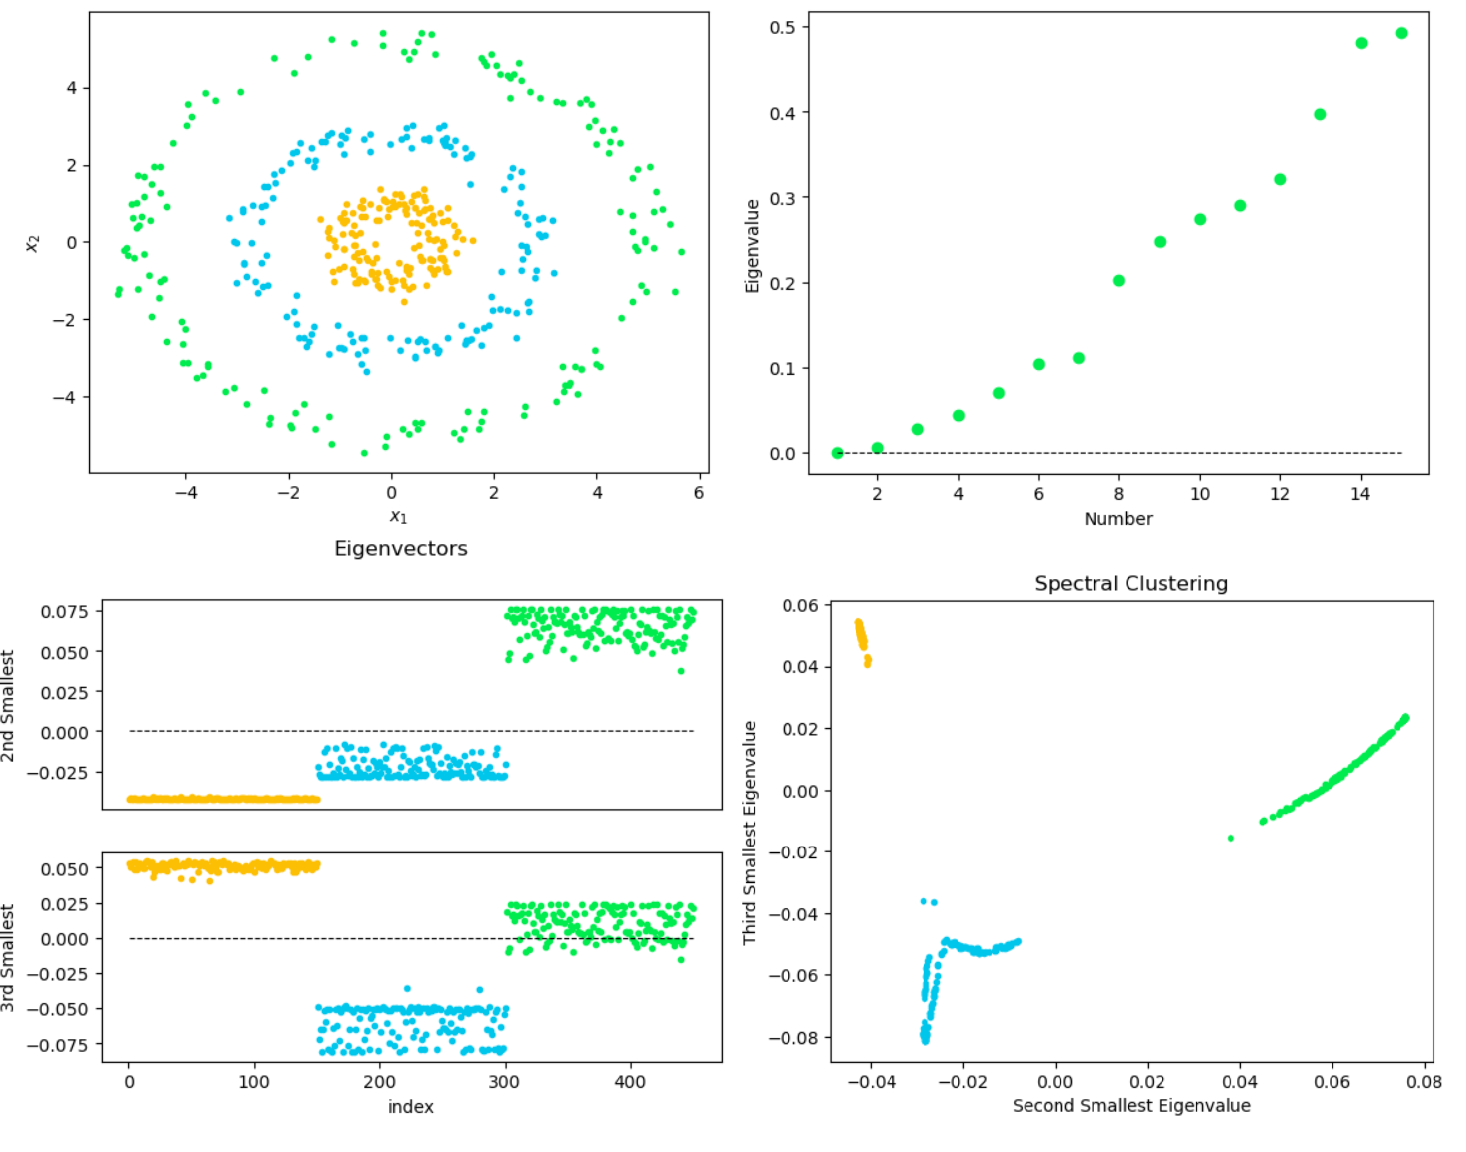
\includegraphics[scale = 0.4]{Graph.png}
    \caption{Replica de la gráfica 14.29 en \textcite{hastie_elements_2009}. En la esquina superior izquierda se aprecia una gráfica de los datos simulados, separados por los colores verde, azul y rojo, de acuerdo al diámetro \(5\), \(2.8\) y \(1\) con el que fueron simulados. En la esquina superior derecha puede encontrar una gráfica con los 15 valores propios más pequeños del Laplaciano, \(L\), de este problema de clasificación espectral. Por otra parte, la gráfica en la esquina inferior izquierda corresponde a las gráficas del segundo y tercer vector propio más pequeños de \(L\). Finalmente, la última gráfica corresponde a una gráfica de dispersión del segundo vector propio más pequeño de \(L\), contra el tercer vector propio más pequeño de \(L\). }
    \label{fig:1}
\end{figure}
\begin{figure}[htb]
    \centering
    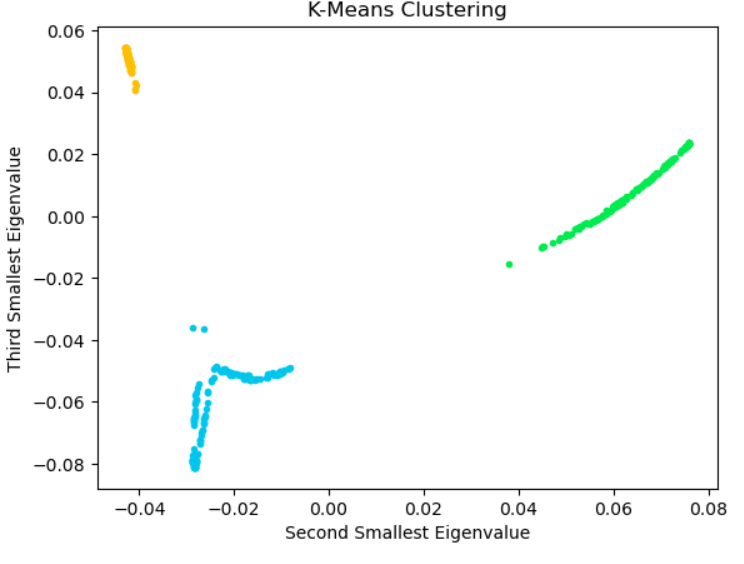
\includegraphics[scale = 0.4]{K-means.png}
    \caption{Agrupación usando \(K\)-means clustering.}
    \label{fig:2}
\end{figure}

\end{solucion}

\section{Anexo.}\label{Anex}
Se enunciara de manera rápida y poco formal versiones de la Ley de Condicionamiento Iterado y la Ley de Probabilidad Total, que fueron de utilidad a lo largo del ejercicio 1.: 
\begin{lem}
Sean \(\overline{Y}_n = (Y_1, \hdots, Y_{n})\) un vector aleatorio absolutamente continuo, \(Z = (Z_{1}, \hdots, Z_{n})\) un vector aleatorio discreto y \(f(\overline{Y}_n,Z)\) la densidad generalizada de \((\overline{Y}_n,Z)\). Entonces
\begin{itemize}
    \item[1.] (Ley de Probabilidad Total.) Se cumple que 
    \[
    f(\overline{Y}_n, Z) = f(\overline{Y}_{n}|Z)f(Z).
    \]
    donde, \(f(\overline{Y}_{n}|Z)\) es la densidad de \(Y\) dado \(Z\) y \(f(Z)\) es la función masa de probabilidades de \(Z\).
    \item[2.] (Ley de Condicionamiento Iterado.) Sea \(f(Y|Z)\) como en el inciso anterior. Si para \(j \in \kis{2,\hdots,n}\) se define \(\overline{Y}_{j-1} =  (Y_{1}, \hdots, Y_{j-1})\), entonces 
    \[
     f(Y_n| \overline{Y}_{n-1},Z)\cdots f(Y_{2}|\overline{Y}_{1},Z)f(Y_{1}|\overline{Y}_{0},Z).
    \]
    donde, para \(j \in \kis{2, \hdots, n-1}\) se tiene que \(f(Y_j| \overline{Y}_{j-1},Z)\) denota la densidad condicional de \(Y_{j}\) dado \(\overline{Y}_{j-1},Z\), mientras que, \(f(Y_{1}|\overline{Y}_{0},Z) = f(Y_{1}|Z)\) denota a la densidad condicional de \(Y_{1}\) dado \(Z\).
\end{itemize}
\end{lem}
Adicionalmente, se enunciará un Lema sobre distribuciones normales que fue empleado a lo largo del Ejercicio.
\begin{lem}\label{lem.1}
Sean \(Y\) una variable aleatoria normal, de media \(\mu\) y varianza \(\sigma^2\), y \(a\) y \(b\) dos números reales. Entonces, \(a Y + b\) posee distribución normal de media \(a \mu + b\) y varianza \(a^2 \sigma^2\). 
\end{lem}


\newpage
\nocite{*}
\printbibliography
\end{document}
